\section{Method}
\label{sec:method}

We frame stagnation detection as window-level binary classification over agent trajectories.
Silver labels are generated via weak supervision from three labeling functions, then used to train and evaluate three detection approaches: structural features, a neural embedding probe, and an LLM-as-judge baseline.
Figure~\ref{fig:pipeline} provides a system overview.

\begin{figure*}[t]
\centering
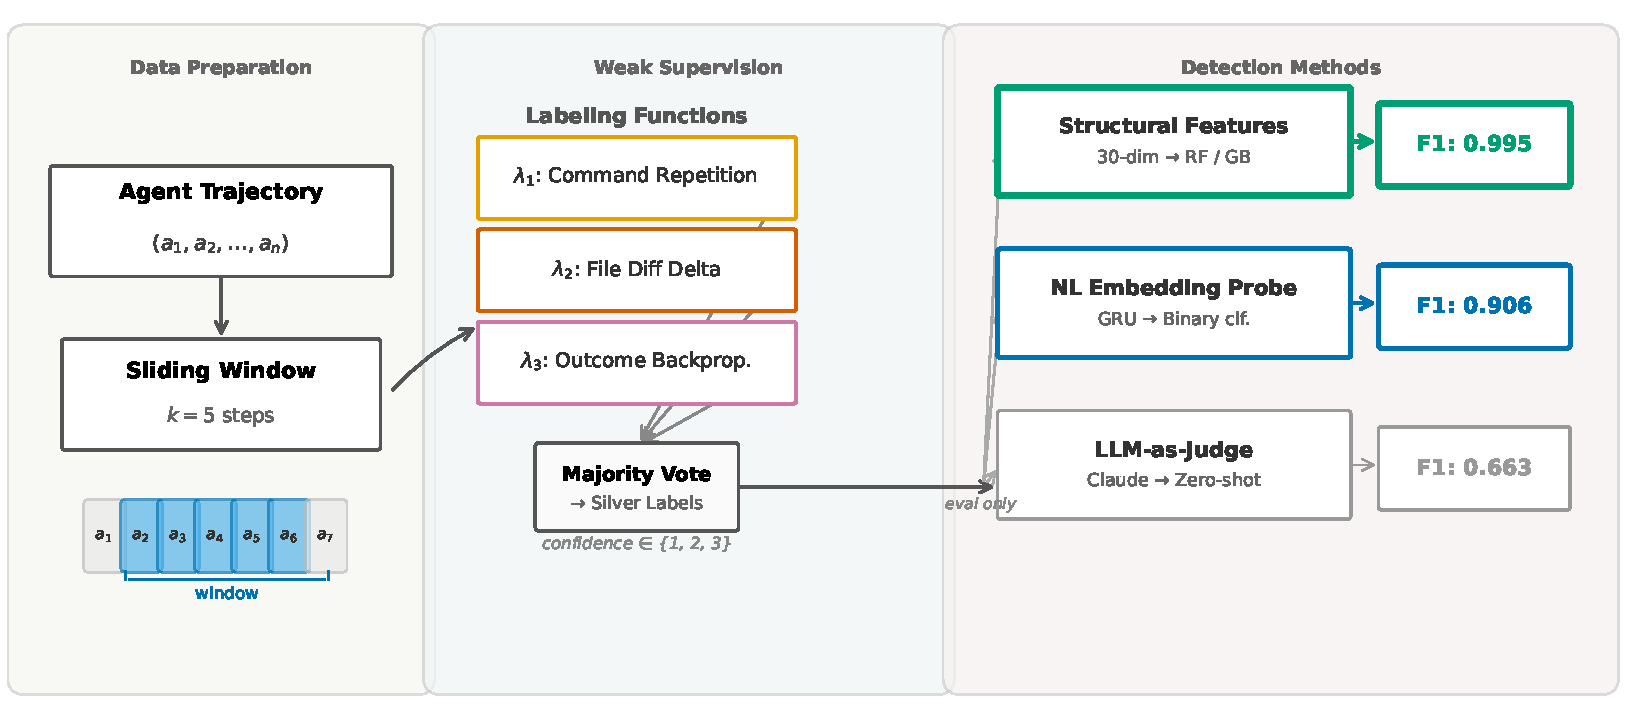
\includegraphics[width=\textwidth]{../../figures/paper/fig_pipeline.pdf}
\caption{System overview. (Left) Agent trajectories are segmented into overlapping windows of $k{=}5$ steps. (Center) Three labeling functions vote on each window; majority vote produces silver labels with confidence 1--3. (Right) Three detection approaches compared: structural features (30-dim), NL embedding probe (GRU), and LLM-as-judge (eval only, not trained on silver labels).}
\label{fig:pipeline}
\end{figure*}

%-------------------------------------------------------------------
\subsection{Problem Formulation}
\label{sec:problem}

Given an agent trajectory $T = (a_1, a_2, \ldots, a_n)$ where each $a_t$ is an action (e.g., a shell command, file edit, or API call), we partition it into overlapping sliding windows $w_i = (a_i, \ldots, a_{i+k-1})$ with window size $k{=}5$ and stride 1.
The task is to assign each window a binary label $y_i \in \{0, 1\}$, where 0 denotes \emph{stagnation} (the agent is stuck or unproductive) and 1 denotes \emph{progress} (the agent is making meaningful headway toward the task goal).

The window formulation offers two advantages over alternatives.
Compared to step-level scoring, windows capture short-range temporal patterns---such as a sequence of repeated failed attempts---that individual actions cannot express.
Compared to trajectory-level labeling, windows provide the granularity needed to pinpoint \emph{when} stagnation begins and ends within a single task attempt, enabling downstream interventions such as early termination or strategy switching.

%-------------------------------------------------------------------
\subsection{Weak Supervision Pipeline}
\label{sec:weak_supervision}

No gold-standard annotations exist for agent stagnation at the window level.
Manual annotation is expensive: each window requires reviewing $k$ actions with full context (command text, outputs, file diffs), taking an estimated 2--3 minutes per window.
We therefore adopt a data programming approach \citep{ratner2016dataprogramming,ratner2017snorkel}: multiple labeling functions (LFs) provide noisy votes that are aggregated into silver labels.
Each LF $\lambda_j : w_i \to \{-1, 0, 1\}$ examines a window and emits a vote: stagnation (0), progress (1), or abstain ($-1$).

\subsubsection{Labeling Functions}
\label{sec:labeling_functions}

We design three LFs that target complementary signals of stagnation (Table~\ref{tab:lf_design}).

\paragraph{Command repetition ($\lambda_1$).}
Computes the proportion of repeated commands within window $w_i$.
A high repetition ratio triggers a stagnation vote, capturing overt repetitive behavior such as re-running failing commands.
This LF fires on 65.6\% of SWE-Agent windows and 92.3\% of OpenHands windows; the elevated OH rate reflects differences in action distributions across agent architectures (\S\ref{sec:cmd_rep_ablation}).

\paragraph{File diff delta ($\lambda_2$).}
Measures the fraction of steps within $w_i$ that produce code modifications (file creates, edits, or deletes).
A low modification frequency triggers a stagnation vote, detecting lack of productive output.
On OpenHands, this LF achieves 87\% correctness on progress windows, making it the most reliable cross-agent signal.

\paragraph{Outcome backpropagation ($\lambda_3$).}
Uses the final task outcome (resolved/unresolved) as distant supervision.
For unresolved tasks, windows in the final portion of the trajectory receive stagnation votes under the assumption that task failure is preceded by a period of unproductive behavior.
Resolved tasks receive progress votes in the corresponding windows.
Unlike $\lambda_1$ and $\lambda_2$, which operate on local window content, $\lambda_3$ propagates a global signal backward through time.
This makes it a form of distant supervision: individually noisy, but complementary to the real-time signals when aggregated.

\begin{table}[t]
\centering
\small
\begin{tabular}{llcc}
\toprule
\textbf{LF} & \textbf{Signal} & \textbf{SWE Fire\,\%} & \textbf{OH Fire\,\%} \\
\midrule
$\lambda_1$ (cmd\_rep)    & Repetition & 65.6 & 92.3 \\
$\lambda_2$ (file\_diff)  & Output     & 57.3 & 42.1 \\
$\lambda_3$ (outcome\_bp) & Outcome    & 23.9 & 19.8 \\
\bottomrule
\end{tabular}
\caption{Labeling function design. Fire\,\% = fraction of windows on which the LF produces a stagnation vote. SWE = SWE-Agent; OH = OpenHands.}
\label{tab:lf_design}
\end{table}

\subsubsection{Label Aggregation}
\label{sec:label_aggregation}

Silver labels are produced by majority vote:
\begin{equation}
y_i = \text{MV}\bigl(\lambda_1(w_i),\; \lambda_2(w_i),\; \lambda_3(w_i)\bigr)
\label{eq:mv}
\end{equation}
We define the confidence of each label as the number of agreeing LFs: $\text{conf}_i = |\{j : \lambda_j(w_i) = y_i\}| \in \{1, 2, 3\}$.
With three binary LFs, majority vote always produces a winner; conf${=}1$ arises when one LF votes opposite to the other two plus abstains differently, producing the most ambiguous labels.
The conf${\geq}$2 subset, where at least two LFs agree on the winning label, serves as the primary evaluation set throughout this work.
This stratification allows us to separately analyze model behavior on high-confidence vs.\ ambiguous windows (\S\ref{sec:main_results}).

%-------------------------------------------------------------------
\subsection{Detection Methods}
\label{sec:detection_methods}

\subsubsection{Structural Features}
\label{sec:structural_features}

We extract a 30-dimensional feature vector from each window, requiring no pretrained model or GPU.
Features span four categories:
(1)~\emph{repetition}: exact command repeat ratio, fuzzy match ratio (Levenshtein-based), and unique command ratio;
(2)~\emph{file operations}: counts of file creates, modifications, and deletions within the window;
(3)~\emph{edit patterns}: edit distances between consecutive actions, capturing how much the agent's behavior changes step-to-step;
(4)~\emph{output statistics}: entropy of command outputs and action type distribution features.
These features are fed to three classifiers: Logistic Regression (LR), Random Forest (RF), and Gradient Boosting (GB).
Because several structural features overlap with the signals used by the labeling functions (e.g., repetition ratios relate to $\lambda_1$), structural classifiers can partially reconstruct the LF voting process.
We discuss this circularity and its implications in \S\ref{sec:main_results}.

\subsubsection{NL Embedding Probe (ProgressProbe)}
\label{sec:progressprobe}

Each action $a_t$ is encoded as a natural language description and embedded using Qwen3-Embedding-0.6B \citep{zhang2025qwen3embedding} into a 1024-dimensional vector.
The $k$ embeddings within a window form a sequence that is processed by a 2-layer GRU \citep{cho2014gru} with hidden size 256 and dropout 0.1.
An attention mechanism \citep{bahdanau2015attention} computes a weighted combination of the GRU hidden states, yielding a single window-level representation.
This representation is passed through a fully connected layer with sigmoid activation for binary classification.
Training uses binary cross-entropy loss with early stopping (patience 5) on a validation set.

The GRU architecture is motivated by the sequential nature of actions within a window: the order in which commands are issued (e.g., repeated failures followed by a different approach) carries diagnostic information that bag-of-embeddings methods discard.
We also evaluate two simpler embedding baselines to isolate the contribution of temporal modeling: (1)~mean-pooled Qwen3 embeddings with logistic regression, and (2)~cosine similarity between consecutive window embeddings with a validation-tuned threshold.

\subsubsection{LLM-as-Judge Baseline}
\label{sec:llm_judge}

We prompt Claude Sonnet in zero-shot mode to classify each window as stagnation or progress, given the textual descriptions of actions within the window.
This baseline serves exclusively for evaluation---it is not used in the silver label pipeline and incurs \$11.66 in API cost for the SWE-Agent test set alone, making it impractical for large-scale labeling.

%-------------------------------------------------------------------
\subsection{Temporal Label Models}
\label{sec:temporal_models}

The three LFs occupy distinct temporal niches relative to stagnation onset (\S\ref{sec:lf_temporal}): $\lambda_1$ leads by ${\sim}2$ steps, $\lambda_2$ is near-concurrent, and $\lambda_3$ lags by ${\sim}7$ steps.
This motivates exploring whether encoding temporal structure into label aggregation can improve over majority vote.

\subsubsection{Time-Varying Weights (TWV)}
\label{sec:twv}

TWV applies Gaussian kernel smoothing to each LF's activation sequence:
\begin{equation}
\tilde{\lambda}_j(t) = \sum_{t'} K_\sigma(t - t') \cdot \lambda_j(t')
\label{eq:twv}
\end{equation}
where $K_\sigma$ is a Gaussian kernel with bandwidth $\sigma$.
Smoothed activations replace raw votes for conf${=}1$ windows (where exactly one LF disagrees), potentially flipping labels in temporally ambiguous regions.
The bandwidth $\sigma$ controls the extent of temporal context: larger values incorporate more distant steps.

\subsubsection{Hidden Markov Models}
\label{sec:hmm}

We model the label sequence as a Hidden Markov Model \citep{safranchik2020linkedhmm} with two hidden states (stagnation, progress) and observations defined by the joint activation pattern of the three LFs.
Transition and emission parameters are estimated via Expectation-Maximization (EM).
The HMM captures temporal persistence---stagnation episodes tend to span multiple consecutive windows---which majority vote, operating independently per window, cannot model.

\subsubsection{Lag-Aware HMM}
\label{sec:lag_hmm}

The standard HMM treats all LFs as synchronous.
Lag-Aware HMM extends this by explicitly modeling each LF's temporal offset: $\lambda_1$ is shifted by $-2$ steps, $\lambda_2$ by $-1$, and $\lambda_3$ by $+7$, estimated from the temporal dynamics analysis (\S\ref{sec:lf_temporal}).
To prevent divergence, we apply two regularization strategies: (1)~\emph{confidence anchoring}, which fixes labels for conf${\geq}$2 windows and restricts EM updates to conf${=}1$ windows; and (2)~a prior strength of 5000 on transition parameters.
These constraints keep the model close to the majority vote baseline while allowing it to resolve temporally ambiguous labels.
The intuition is that aligning each LF's activation to its natural temporal role should produce cleaner emission estimates and, consequently, more accurate Viterbi decodings on ambiguous windows.
